\documentclass[a4paper,11pt]{article}
\usepackage[T1]{fontenc}
\usepackage[utf8]{inputenc}
\usepackage{graphicx}
\usepackage{amsmath}
\usepackage{amsfonts}
\usepackage[brazilian]{babel}
\usepackage[left=2.5cm,right=2.5cm,top=2.0cm,bottom=1.5cm]{geometry}
\usepackage[hidelinks]{hyperref}
\usepackage{indentfirst}
\usepackage{caption}
\usepackage{subcaption}
\usepackage{algorithm}
\usepackage{algpseudocode}
\usepackage{listings}

\date{}
\author{Lucas Magno \\ 7994983}
\title{Exercício Programa 3 \\ Matrizes Ortogonais e o Problema de Quadrados Mínimos}

\begin{document}
    \maketitle

    \section*{Introdução}
        Este EP consiste em se resolver um sistema linear sobredeterminado na forma
        $$ Ax = b $$
        onde
        \begin{align*}
            A & \in \mathbb{R}^{n\times m}\\
            x & \in \mathbb{R}^{m} \\
            b & \in \mathbb{R}^{n}
        \end{align*}

        a fim de minimizar a norma do resíduo, ou, equivalentemente, sua norma ao quadrado, dada por
        \begin{align*}
            \| r \|_2^2 &= \| b - Ax \|_2^2 \\
                                 &= \sum_{i = 1}^n (b_i - (Ax)_i)^2 \\
                                 &= \sum_{i = 1}^n r_i^2
        \end{align*}

        Ou seja, o problema se resume em encontrar $x$ que minimize os $r_i^2$, o que dá o nome ao Método dos Mínimos Quadrados.

    \section*{Matrizes Ortogonais}
        Para tal, vale a pena o estudo de matrizes ortogonais, que são definidas como qualquer matriz $Q$ tal que
        $$ Q^TQ = I$$
        ($Q^T$ também é ortogonal).

        E portanto, como se verifica facilmente para qualquer vetor ou matriz $x$
        $$ \| Qx \|_2 = \| x \|_2$$

        Ou seja, podemos utilizar matrizes ortogonais para transformar o sistema na forma
        $$ Q^TAx = Q^Tb$$

        cujo resíduo
        $$ r = Q^Tb - Q^TAx$$

        tem a mesma norma que o sistema original
        $$ \|r\|_2 = \|Q^T(b - Ax)\|_2 = \|b - Ax\|_2$$

        Ou seja, podemos transformar o sistema em um mais simples de se resolver, com a garantia de que as soluções são a mesma.
    \newpage
    \section*{Refletores de Householder}

        Uma transformação ortogonal interessante para o nosso caso é uma reflexão de Householder, que permite a seguinte transformação de um determinado
        vetor $x \in \mathbb{R}^n$
        $$ Q\begin{bmatrix}
                x_1 \\
                x_2 \\
                \vdots \\
                x_n
            \end{bmatrix}
            \rightarrow
            \begin{bmatrix}
                -\tau  \\
                0      \\
                \vdots \\
                0
            \end{bmatrix}$$
        onde $Q$ é o refletor e $\tau = \pm \|x\|_2$.
        Melhor ainda, sua construção é bem simples, dada por
        $$ Q = I - \gamma u u^T $$
        com
        $$
            \gamma = \frac{x_1 + \tau}{\tau}\text{ , }
            u =
            \begin{bmatrix}
                1 \\
                x_2/(x_1+\tau) \\
                \vdots         \\
                x_n/(x_1+\tau)
            \end{bmatrix}
        $$
        então só $\gamma$ e $u$ precisam ser armazenados, e não a $Q$ inteira.\footnote{Também não é difícil verificar que $Q$ é simétrica e $Q = Q^T$.}

    \section*{Decomposição QR}
        Portanto, escolhendo a transformação de forma a realizar isso na primeira coluna da matriz A, com norma $\tau_1$ e a chamando de $Q_1$, temos
        $$ Q_1
        \begin{bmatrix}
            a_{11} & a_{12} & \dots & a_{1m} \\
            a_{21} & a_{22} & \dots & a_{2m} \\
            \vdots & \vdots & \ddots & \vdots \\
            a_{n1} & a_{n2} & \dots & a_{nm} \\
        \end{bmatrix}
        \rightarrow
        \left[
        \begin{array}{c|ccc}
            -\tau_1  & a_{12}^* & \dots & a_{1m}^* \\ \hline
                  0 &  &  &  \\
            \vdots &  & A_2 &  \\
                  0 &  &  &  \\
        \end{array}\right] $$

        Podemos ainda escolher uma nova transformação $\hat{Q}_2$ para realizar o mesmo na primeira coluna de $A_2$, mas precisamos compô-la com a identidade para que ela aja somente em $A_2$, não alterando o restante de $A$.
        Então
        $$
        Q_2 =
        \left[
        \begin{array}{c|ccc}
            I_1 & 0 & \dots & 0 \\ \hline
            0 & &  & \\
            \vdots & & \hat{Q}_2 & \\
            0 & &  & \\
        \end{array} \right]
        $$
        aí teremos
        $$Q_2Q_1
        \begin{bmatrix}
            a_{11} & a_{12} & \dots & a_{1m} \\
            a_{21} & a_{22} & \dots & a_{2m} \\
            \vdots & \vdots & \ddots & \vdots \\
            a_{n1} & a_{n2} & \dots & a_{nm} \\
        \end{bmatrix}
        \rightarrow
        \left[
        \begin{array}{cc|ccc}
            -\tau_1  & a_{12}^* & a_{13}^* & \dots & a_{1m}^* \\
                  0  & -\tau_2  & a_{23}^* & \dots & a_{2m}^* \\ \hline
                  0  &       0  &          &       &          \\
            \vdots   &  \vdots  &          &  A_3  &          \\
                  0  &       0  &          &       &          \\
        \end{array}\right] $$

        Escolhendo uma reflexão para cada coluna de $A$, poderíamos fazer
        $$ Q_m\dots Q_1A =
        \begin{bmatrix}
            R \\
            0
        \end{bmatrix}
        $$
        com $R \in \mathbb{R}^{m\times m}$ triangular superior.
        Na prática, no entanto, as colunas de $A$ nem sempre são linearmente independentes, e eventualmente alguma subcoluna terá norma nula (portanto $\tau = 0$), tornando a $R$ singular, o que não permitiria seu uso para resolver o sistema.

        Para evitar isso, organizar as colunas de $A$ de forma a manter as subcolunas de maiores normas à esquerda, isto é, antes de escolher cada $Q_k$ ($k = 1\dots m$), escolher a subcoluna de maior norma de $A_k$ e trocá-la com a primeira, de forma que os $\tau_k$ fiquem organizados em ordem decrescente.

        Assim, se no passo $r+1$ a maior norma das subcolunas de $A_{r+1}$ é zero, então todos os elementos dessa submatriz são nulos e temos
        $$ Q_r\dots Q_1AP = R =
        \begin{bmatrix}
            R_{11} & R_{22} \\
                 0 &      0
        \end{bmatrix}$$

        onde $R_{11} \in \mathbb{R}^{r\times r}$ é triangular superior e não-singular.\footnote{Alterar as colunas de $A$ durante os passos é equivalente a ter multiplicado ela inicialmente por uma matriz de permutação $P$.}

        Definindo
        $$ Q^T = Q_r \dots Q_1 $$
        temos
        $$ AP = QR $$
        que é a decomposição QR da matriz $A$ com pivotamento.

    \section*{Solução do Problema de Mínimos Quadrados}
        Voltando ao sistema original,
        \begin{align*}
            APP^{-1}x &= b \\
            QRP^{-1}x &= b \\
             RP^{-1}x &= Q^Tb \\
        \end{align*}

        E a resolução do sistema se resume a
        \begin{align*}
            c        &= Q^Tb \\
            R\hat{x} &= c \\
            x        &= P\hat{x}
        \end{align*}

        Sabendo a forma de $R$, no entanto, podemos calcular o resíduo \footnote{$\hat{x}_1, \hat{c} \in \mathbb{R}^{r}$}
        \begin{align*}
            r &=
            \begin{bmatrix}
                R_{11} & R_{22} \\
                     0 &      0
            \end{bmatrix}
            \begin{bmatrix}
                \hat{x}_1 \\
                \hat{x}_2
            \end{bmatrix}
            -
            \begin{bmatrix}
                \hat{c} \\
                d
            \end{bmatrix} \\
            &=
            \begin{bmatrix}
                R_{11}\hat{x}_1 + R_{22}\hat{x}_2 - c \\
                d
            \end{bmatrix}
        \end{align*}
        cuja norma ao quadrado é
        $$ \|r\|_2^2 = \|R_{11}\hat{x}_1 + R_{22}\hat{x}_2 - \hat{c}\|_2^2 + \|d\|_2^2$$

        que é quem queremos minimizar. Fica claro que não podemos alterar o termo $\|d\|_2^2$, mas podemos escolher $\hat{x}_1$ e $\hat{x}_2$ de forma a zerar o primeiro termo. Ou seja

        $$ R_{11}\hat{x}_1 = \hat{c} - R_{22}\hat{x}_2$$
        o que tem infinitas soluções, dependendo da escolha dos termos. Como é arbitrário, podemos pegar simplesmente $\hat{x}_2 = 0$ e o segundo passo da solução ($R\hat{x} = c$) se reduz resolver o sistema triangular superior não-singular
        $$ R_{11}\hat{x}_1 = \hat{c} $$
        e o resíduo se torna
        $$ \|r\|_2 = \|d\|_2 $$

    \section*{O programa}
        Esses métodos foram então implementados em um programa em C, que permite resolver um dado sistema sobredeterminado ou então ajustar um polinômio de certo grau a um dado conjunto de pontos.

        Ou seja, há duas formas de invocar o programa, cada uma com um tipo de arquivo de entrada diferente.

        \subsection*{Sistema sobredeterminado qualquer}
            Resolve o sistema
                $$ Ax = b $$
            com $A \in \mathbb{R}^{n\times m}$ e $b \in \mathbb{R}^n$, bem como essas dimensões, fornecidas num arquivo de entrada no seguinte formato\footnote{Vale notar que as matrizes devem ser escritas ordenadas por linhas.}
        \begin{lstlisting}[mathescape, frame=single, caption={Formato do arquivo de entrada com um sistema sobredeterminado}]
        n m
        $a_{11}$
        $a_{12}$
        $\vdots$
        $a_{n,m-1}$
        $a_{nm}$
        $b_1$
        $\vdots$
        $b_n$
        \end{lstlisting}

            E o programa em si é invocado na forma

        \begin{lstlisting}
        $ EP3 sys filename
        \end{lstlisting}


        \subsection*{Ajuste polinomial a um conjunto de pontos}
            Dado um conjunto de pontos
                $$ (t_i, b_i),\quad i = 1\dots n$$
            ajusta um polinômio de grau $m-1$ a esses pontos por mínimos quadrados.

            Ou seja, monta a matriz de Vandermonde do sistema
            $$ A =
            \begin{bmatrix}
                1 & t_1 & t_1^2 & \dots & t_1^{m-1} \\
                1 & t_2 & t_2^2 & \dots & t_2^{m-1} \\
                \vdots & \vdots &\vdots & \ddots & \vdots   \\
                1 & t_n & t_n^2 & \dots & t_n^{m-1} \\
            \end{bmatrix}$$
            e a utiliza para resolver o sistema
            $$ Ax = b$$
            em que $x$ é o vetor de coeficientes do polinômio que melhor ajusta os pontos, isto é
            $$ p(t) = x_1 + x_2t + x_3t^2 + \dots + x_mt^{m-1}$$

            \newpage
            Os dados e as dimensões devem ser fornecidos no arquivo de entrada no formato
        \begin{lstlisting}[mathescape, frame=single, caption={Formato do arquivo de entrada com um conjunto de pontos}]
        n m
        $t_{1}\, b_{1}$
        $t_{2}\, b_{2}$
        $\vdots$
        $t_{n}\, b_{n}$
        \end{lstlisting}

        e o programa é invocado na forma

        \begin{lstlisting}
        $ EP3 data filename
        \end{lstlisting}


        Em ambos casos, o vetor solução $x$ é escrito para um arquivo de saída com o mesmo nome do de entrada, \texttt{filename}, mas com extensão \texttt{.out}.
        Além disso, no caso de ser um conjunto de dados com um polinômio ajustado, é salvo em um arquivo \texttt{pdf} o plot dos dados sobrepostos ao polinômio encontrado.

    \section*{Detalhes de implementação}
        Vale a pena mencionar alguns detalhes que influenciam na eficiência do programa que foram implementados.

        \subsection*{Normalização}
            Sempre ao se realizar a soma de pontos flutuantes arbitrários há o perigo de overflow, contaminando o restante da computação. Esse risco é ainda maior no cálculo de normas, que é parte central do algoritmo aqui implementado.

            Portanto, para evitar isso, pode-se reescalar os elementos de um vetor de forma que o máximo deles tenha valor 1, calcular a norma, e reescalar de volta, o que elimina a chance de overflow, já que todos os elementos têm valor baixo.

            No entanto, isso teria que ser feito a cada norma calculada e seria necessário um vetor auxiliar para guardar cada fator de escala. Então se escolheu reescalar a matriz $A$ inteira por seu maior elemento, evitando-se o overflow em todas as operações seguintes e no final simplesmente se reescala o vetor $b$ também para se obter um sistema equivalente e então resolvê-lo, sendo necessário o armazenamento de um único escalar.

        \subsection*{Normas}
            Novamente, o cálculo de normas é parte central do algoritmo aqui, então uma preocupação com sua eficiência é necessária.

            A cada passo, deve ser escolhida a subcoluna de maior norma, o que implicaria no cálculo das normas de todas subcolunas, que claramente é muito custoso.

            Entretanto, calculando-se as normas das colunas completas e guardando seus quadrados num vetor auxiliar, podemos obter a norma de qualquer subcoluna simplesmente removendo a contribuição dos elementos superiores.

            Ou seja, como a norma de uma dada coluna $y$ é
            $$ \tau_1^2 = y_1^2 + y_2^2 + \dots + y_n^2 $$
            a norma da primeira subcoluna (sem o elemento $y_1$) é dada por
            \begin{align*}
                \tau_2^2 &= y_2^2 + \dots + y_n^2 \\
                         &= \tau_1^2 - y_1^2
            \end{align*}
            poupando grande parte das operações.

    \section*{Exemplo}
        Para ilustrar o funcionamento do programa, foi escolhido um conjunto de dados colhidos durante um experimento de física experimental, que buscava encontra a razão carga-massa, ou carga reduzida, do elétron, através do Método da Hélice de Busch.

        Esse método consiste inserir um feixe de elétrons gerado num tudo de raios catódicos com uma dada tensão aceleradora num campo magnético por sua vez gerado por um solenoide com uma dada corrente.

        Variando-se ambas tensão e corrente, pode-se alterar a posição em que os diversos elétrons atingem um certo anteparo a uma dada distância da origem do feixe.

        No entanto, para certos valores de tensão e corrente, todas as trajetórias convergem num único ponto no anteparo e nesse caso vale a expressão

        $$ V = \alpha \frac{e}{m}I^2 $$
        em que $V$ é a tensão do tubo de raios catódicos, $I$ é a corrente no solenoide, $\alpha$ é uma costante composta por vários dados do experimento (a distância até o anteparo, por exemplo), $e$ é o valor absoluto carga do elétron e $m$ é sua massa.

        Assim, foram registrados diversos valores de $V$ em e $I^2$ para os quais a expressão era válida e a eles ajustado um polinômio de primeiro grau, a fim de se encontrar a todo o coeficiente que contém a carga reduzida.

        Utilizando esses dados, obtemos com o programa atual o ajuste
        \begin{figure}[h]
            \caption{Tensão em função do quadrado da corrente para os quais as trajetórias dos feixes de elétron convergem}
            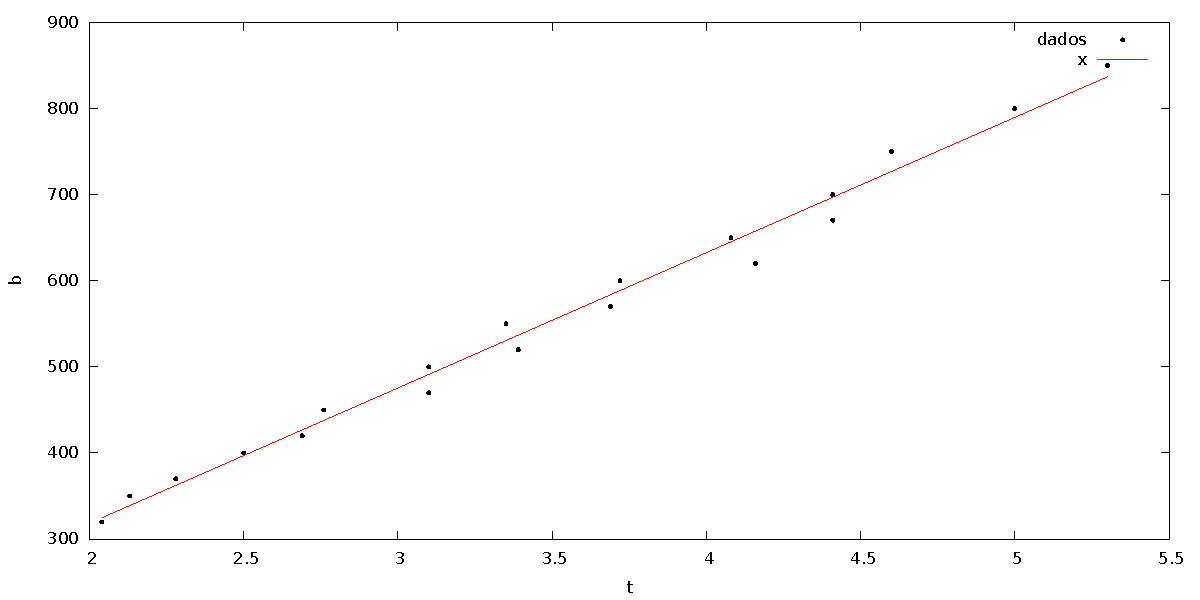
\includegraphics[width=\textwidth]{Dados/dados2.pdf}
        \end{figure}

        em que $b$ neste caso é a tensão, em volts ($V$), $t$ é o quadrado da corrente, em ampères quadrados ($A^2$) e o polinômio ajustado foi
        $$ p(t) = x_1 + x_2t $$

        \newpage
        Para o coeficiente angular (termo que multiplica $t = I^2$) foi encontrado
        $$ x_2 = \alpha \frac{e}{m} \approx 1.57\times 10^2 \frac{V}{A^2}$$

        Levando em conta a constante $\alpha$ (que não é de interesse aqui), podemos obter
        $$ \frac{e}{m} \approx 1.46\times 10^{11} \frac{C}{Kg} $$

        que é próximo do valor correto medido
        $$ \frac{e}{m} = 1.76\times 10^{11} \frac{C}{Kg} $$

        e está dentro do intervalo de confiança quando se utilizam as incertezas.\footnote{Que não foram consideradas aqui por limitação do algoritmo, mas foi mantido o número de algarismos significativos do experimento original.}
    \section*{Conclusão}
\end{document}
